%!TeX root=../tese.tex
%("dica" para o editor de texto: este arquivo é parte de um documento maior)
% para saber mais: https://tex.stackexchange.com/q/78101/183146

%% ------------------------------------------------------------------------- %%

%Recomendação WILL: 
% Ao invés de mecânica colocar design : X
% TD Mencionar Tabelas : X
% TD Mencionar Figuras 4.1 , 4.2, 4.4, 4.5 : X
% SS Mencionar Tabelas : 4.3,  4.4: X
% SS Mencionar Figuras:  4.7, 4.8, 4.9, 4.10, 4.11, 4.12:X

\chapter{Design dos jogos}
\label{cap:mecanica-dos-jogos}

O desenvolvimento dos jogos foi focado em características comuns entre si, para possibilitar o uso do mesmo algoritmo genético, minimizando a necessidade de ajustes no código. A implementação inicial foi feita no \textit{Tower Defense}, e em seguida no \textit{Space Shooter}.

%% ------------------------------------------------------------------------- %%
\section{Tower Defense}
\label{sec:mj-td}

\subsection{O jogo}
\label{sub-sec:jogo-td}

O jogo \textit{Tower Defense} \footnote{Repositório contendo o jogo: { \url{https://github.com/raktanaka/tccTD} - 21/12/2021}} consiste em mapa com dois caminhos a serem percorridos por tanques inimigos e oferece ao jogador duas torres para impedir que os tanques completem seu trajeto. O início do percurso é na esquerda da tela, terminando na direita, conforme visto na Figura \ref{fig:td-inicial}.

\begin{figure}
  \centering
  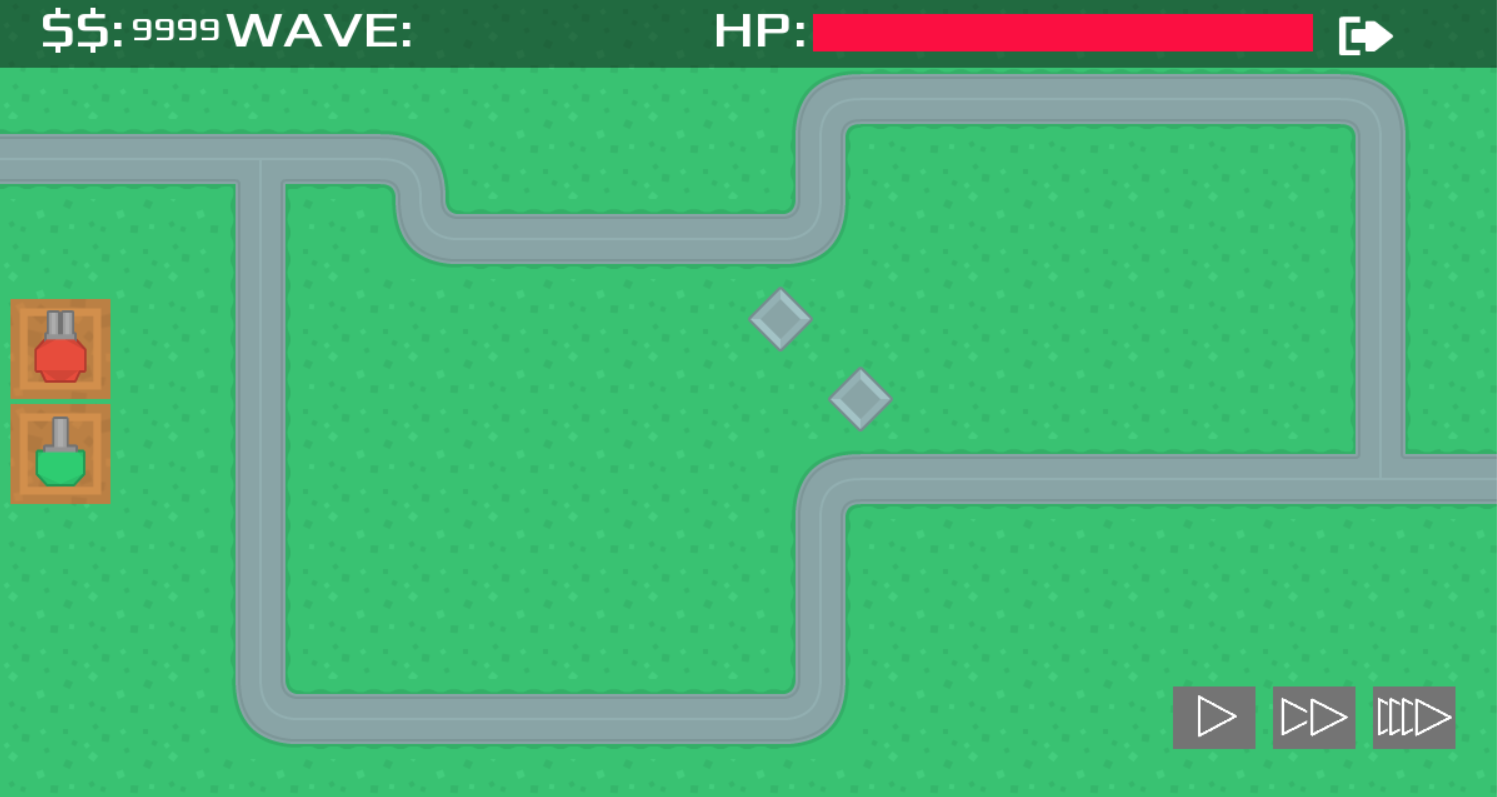
\includegraphics[width=\textwidth]{td/Mapa_inicial_tDD.png}
  \caption{Tela Inicial. Imagem retirada do próprio jogo.\label{fig:td-inicial}}
\end{figure}

Antes de apertar o botão \textit{Play}, o jogador pode colocar quantas e quaisquer torres desejar em áreas livres do mapa. Iniciando a partida, uma onda de 12 tanques começa a percorrer o caminho, inicialmente 6 para cada percurso, conforme a Figura \ref{fig:td-exemplo}. Posteriormente, o algoritmo genético gerencia a rota. Ao lado do botão \textit{Play} estão botões que aceleram a execução do jogo em duas vezes e oito vezes, para facilitar a coleta de dados para os testes.

As duas torres disponíveis oferecem diferentes áreas de alcance para detecção de tanques, apresentadas nas Figuras \ref{fig:td-range-gree} e \ref{fig:td-range-red} e quantidade de dano que podem causar, como esta descrito na Tabela \ref{tab:dados_torres}. Cada inimigo que atinge o objetivo produz dano ao jogador, que possui 100 pontos de vida, mostrado pela barra \textit{HP} na tela. A região também mostra os recursos monetários disponíveis ao jogador - que não está implementado - e a onda atual; o jogo somente termina quando acaba o \textit{HP} do jogador.

\begin{figure}
  \centering
  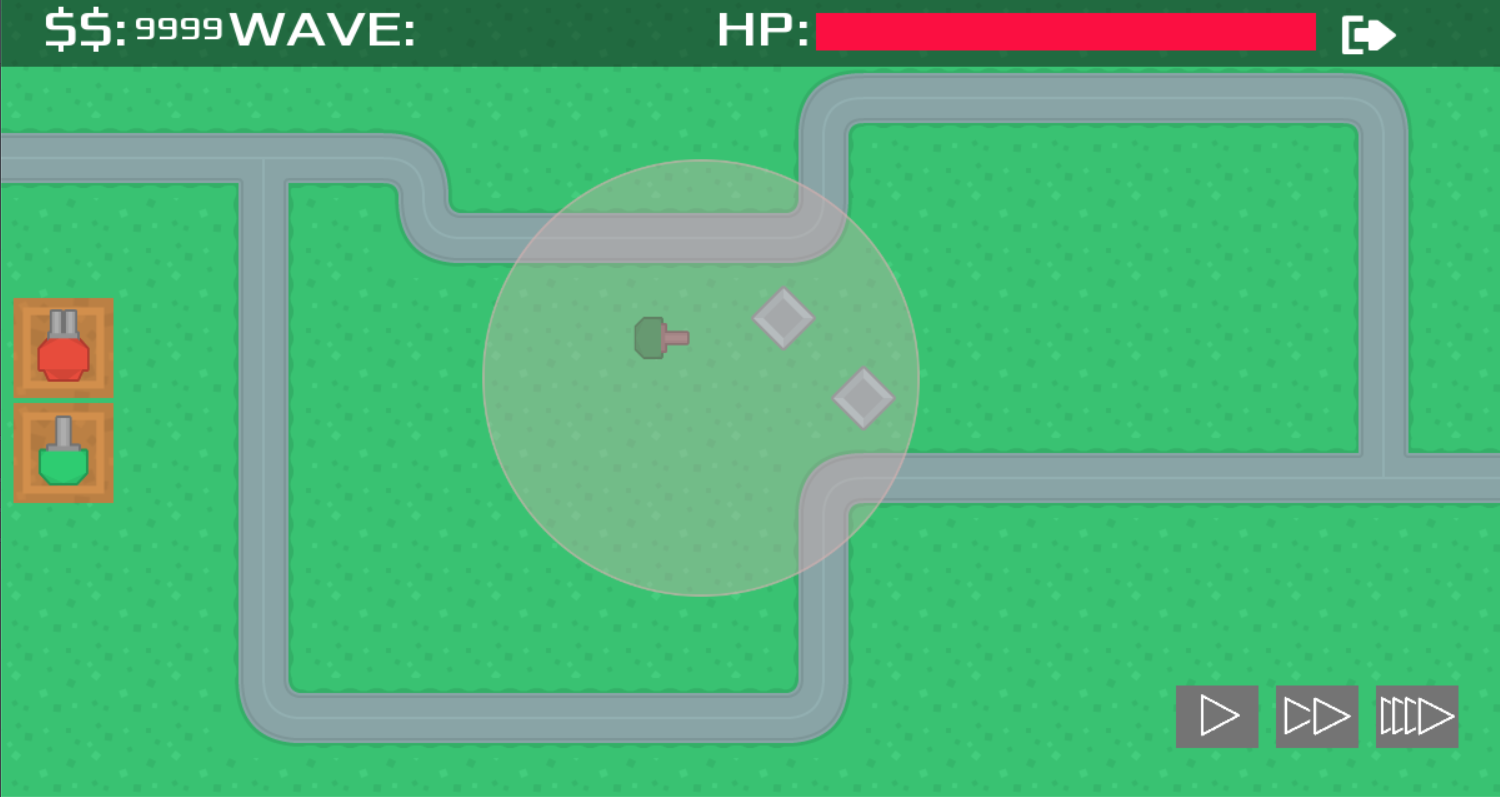
\includegraphics[width=0.8\textwidth]{td/range_green_tower.png}
  \caption{Área de detecção torre verde. Imagem retirada do próprio jogo.\label{fig:td-range-gree}}
\end{figure}

\begin{figure}
  \centering
  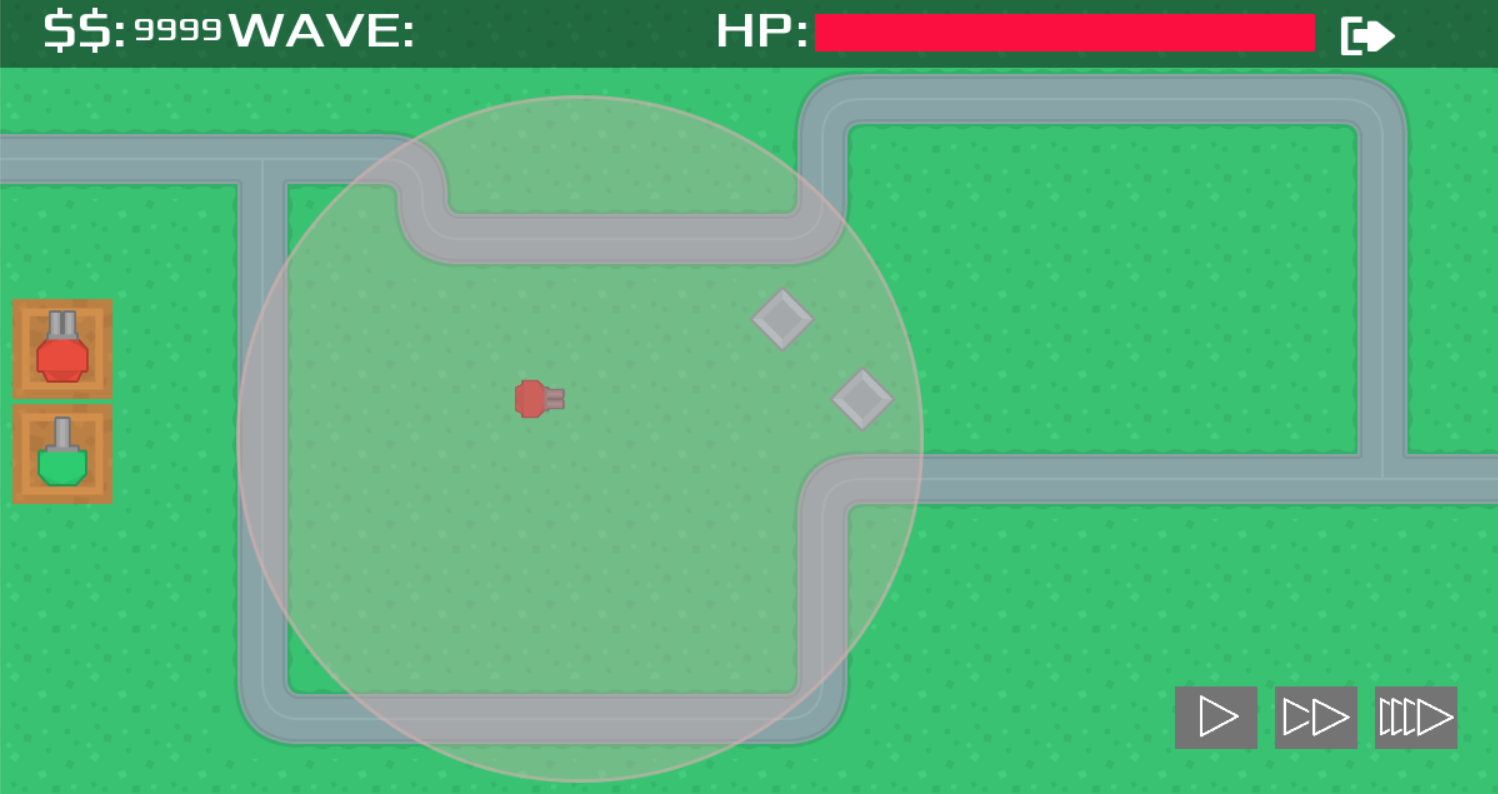
\includegraphics[width=0.8\textwidth]{td/range_red_tower.png}
  \caption{Área de detecção torre vermelha. Imagem retirada do próprio jogo.\label{fig:td-range-red}}
\end{figure}

\begin{table}[H]
\caption{Dano das torres no Tower Defense.\label{tab:dados_torres}}
\begin{tabular}{c|ccc}

               & velocidade de tiro  & dano   & alcance\\ \hline
Torre Verde    & 55                  & 25     &  350 \\
Torre Vermelha & 70                  & 15     &  550       

\end{tabular}
\end{table}


\begin{figure}
  \centering
  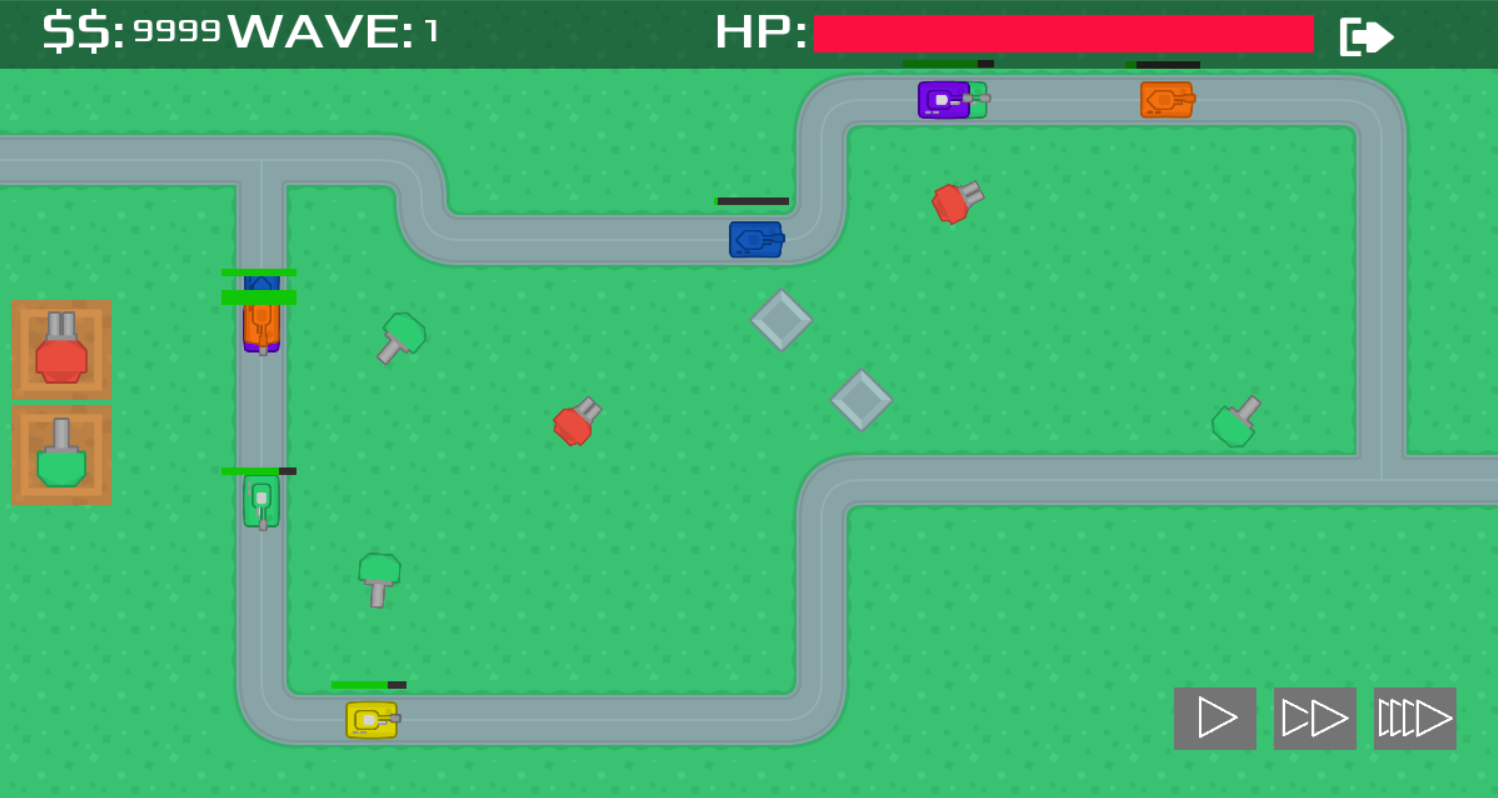
\includegraphics[width=\textwidth]{td/exemplo de execução TDD.png}
  \caption{Exemplo de uma execução do jogo. Imagem retirada do próprio jogo.\label{fig:td-exemplo}}
\end{figure}


Existem 6 tipos de tanques diferentes, descritos na Figura \ref{fig:figure-tipos-tanque}. Cada tipo de tanque possui 2 características, sendo elas velocidade e dano causado ao jogador, cujo os valores variam conforme o tipo, visto a Tabela \ref{tab:tank-dmg}. 

\begin{figure}
     \centering
     \begin{subfigure}[b]{0.2\textwidth}
         \centering
         
\includegraphics[width=\textwidth]{td/tank_blue.png}
         \caption{tank blue}
         \label{fig:td-tank-blue}
     \end{subfigure}
     \hfill
     \begin{subfigure}[b]{0.2\textwidth}
         \centering
         
\includegraphics[width=\textwidth]{td/tank_green.png}
         \caption{tank green}
         \label{fig:td-tank-green}
     \end{subfigure}
     \hfill
     \begin{subfigure}[b]{0.2\textwidth}
         \centering
         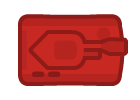
\includegraphics[width=\textwidth]{td/tank_red.png}
         \caption{tank red}
         \label{fig:td-tank-red}
     \end{subfigure}
     
     \begin{subfigure}[b]{0.2\textwidth}
         \centering
         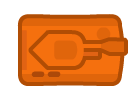
\includegraphics[width=\textwidth]{td/tank_orange.png}
         \caption{tank orange}
         \label{fig:td-tank-orange}
     \end{subfigure}
     \hfill
     \begin{subfigure}[b]{0.2\textwidth}
         \centering
         
\includegraphics[width=\textwidth]{td/tank_purple.png}
         \caption{tank purple}
         \label{fig:td-tank-purple}
     \end{subfigure}
     \hfill
     \begin{subfigure}[b]{0.2\textwidth}
         \centering
         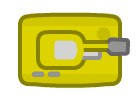
\includegraphics[width=\textwidth]{td/tank_yellow.png}
         \caption{tank yellow}
         \label{fig:td-tank-yellow}
     \end{subfigure}     
     \caption{Tipos de tanques}
     \label{fig:figure-tipos-tanque}
\end{figure}

\newpage

\begin{table}
\caption{Dano de cada tanque no Tower Defense}
\begin{tabular}{c|cc}
            & velocidade & dano   \\ \hline
tank blue   & 55    & 55         \\
tank green  & 70    & 45         \\
tank red    & 80    & 15          \\
tank orange & 120   & 5           \\
tank purple & 90    & 15          \\
tank yellow & 150   & 5           
\end{tabular}
\label{tab:tank-dmg}
\end{table}

Ficam definidas como Norte e Sul as rotas disponíveis, na Figura \ref{fig:td-rota}.

\begin{figure}
  \centering
  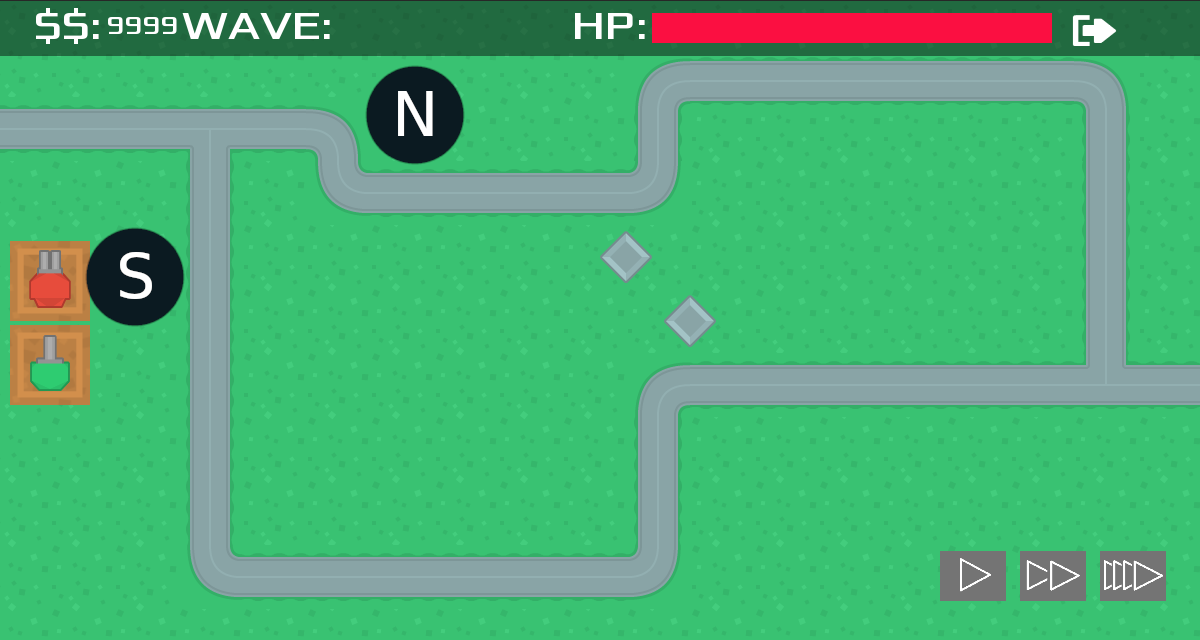
\includegraphics[width=\textwidth]{td/td_positions.png}
  \caption{Definição das rotas Norte e Sul. Imagem retirada do jogo e editada.\label{fig:td-rota}}
\end{figure}

\subsection{Mecânica de Resistência}
\label{sub-sec:mecanica-de-resistencia}

No jogo de \textit{Tower Defense} também foi adicionado um sistema de resistência nos tanques, cada Tanque possui resistência contra Torres de \textbf{mesma cor} e recebem dano reduzido pela metade dos mesmos. Segue um pseudocódigo da implementação do tanque ao receber dano de uma torre.

\begin{programruledcaption}{Sistema de Resistência TD.\label{prog:resistencia-TD}}
  \begin{lstlisting}[
    language={[brazilian]pseudocode},
    style=pseudocode,
    style=wider,
    functions={},
    specialidentifiers={},
  ]
        // x = tanque que recebe o dano
        // damage = quantidade total de dano recebido
        // color\_tower = cor da torre que disparou no tanque.
        func on_hit(x, damage, color_tower):
            // color (x) = cor do tanque \textbf{x}
            //  hp(x) = hp atual de x.
	        se color (x) = color_tower:
		        hp (x) -= damage / 2
		
        	senao:
        		hp (x) -= damage
        fim
  \end{lstlisting}
\end{programruledcaption}


\newpage
%% ------------------------------------------------------------------------- %%
\section{Space Shooter}
\label{sec:mj-ss}

O jogo \textit{Space Shooter}\footnote{Repositório contendo o jogo { \url{https://github.com/RGPRafael/godot} - 21/12/2021}} consiste em uma nave que o jogador pode mover livremente em um espaço 2D, onde este deve sobreviver a ondas de asteroides que partem de diferentes posições da tela em sua direção. O jogador além de esquivar, pode eliminar os asteroides por meio de disparos com o \textit{mouse}. 

\begin{figure}
  \centering
  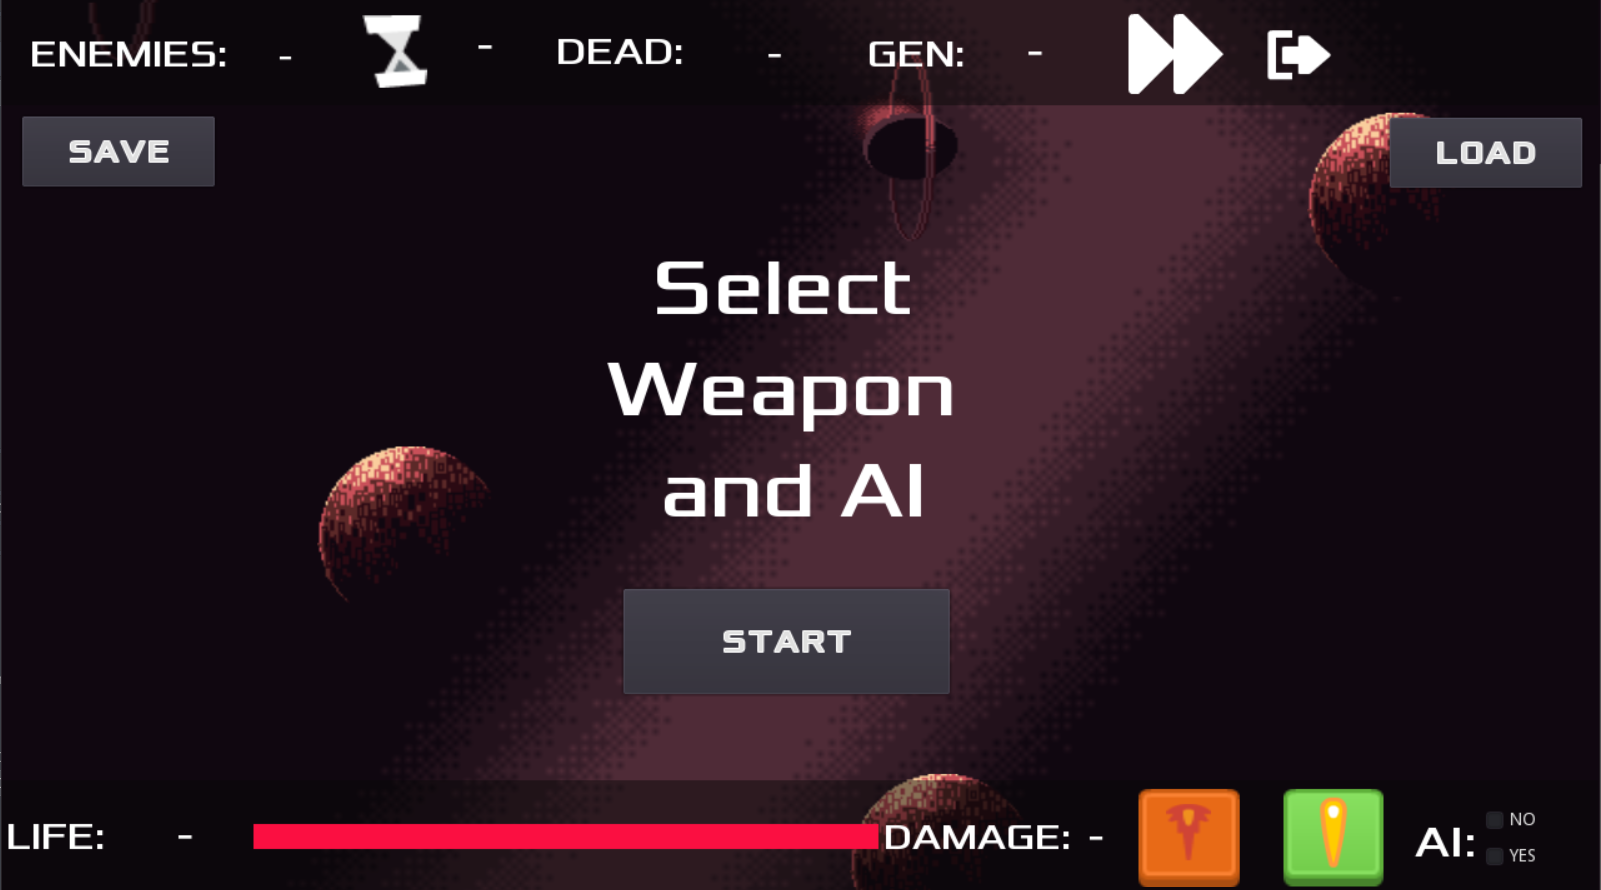
\includegraphics[width=\textwidth]{ss/Tela_inicial_space_shooter.png}
  \caption{Tela inicial. Imagem retirada do próprio jogo.\label{fig:ss-start}}
\end{figure}

Existem dois tipos de disparos que o jogador pode usar para sua defesa, cada um com características diferentes. No começo do jogo é requisitado que o jogador escolha qual tipo de disparo irá utilizar, conforme as Figuras \ref{fig:ss-start} e \ref{fig:ss-disparos}.

\begin{figure}
     \centering
     \begin{subfigure}[b]{0.15\textwidth}
         \centering
         
\includegraphics[width=\textwidth]{ss/Disparo_.png}
         \caption{Disparo}
         \label{fig:ss-disparo}
     \end{subfigure}
     \begin{subfigure}[b]{0.15\textwidth}
         \centering
         
\includegraphics[width=\textwidth]{ss/Disparo1_.png}
         \caption{Disparo1}
         \label{fig:ss-disparo1}
     \end{subfigure}
     \caption{Disparos}
     \label{fig:ss-disparos}
\end{figure}

\begin{table}
\caption{Dano dos tiros no Space Shooter}
\begin{tabular}{c|cc}
          & Velocidade de Tiro & Dano \\ \hline
Disparo   & 1200  & 15     \\
Disparo 1 & 600   & 30    
\end{tabular}
\label{tab:tiro=-ss}
\end{table}

Existem dois tipos de \textit{player} automáticos disponíveis para escolha, caso o jogador marque a opção \textit{'yes'} na barra inferior, próximo ao texto \textit{'AI'}, como pode se observar na Figura \ref{fig:ss-player-ai}. Tais \textit{players} foram desenvolvidos com o intuito de auxiliar no projeto, e na realização dos testes e coleta de dados. Uma delas faz com que a nave transite da direita para esquerda em um intervalo de cinco minutos, a outra opção faz com que a nave fique parada no meio da tela, em ambos atirando no inimigo mais próximo que detectar, de forma a destruir o asteroide que vem em sua direção ou ser atingida.  

\begin{figure}
  \centering
  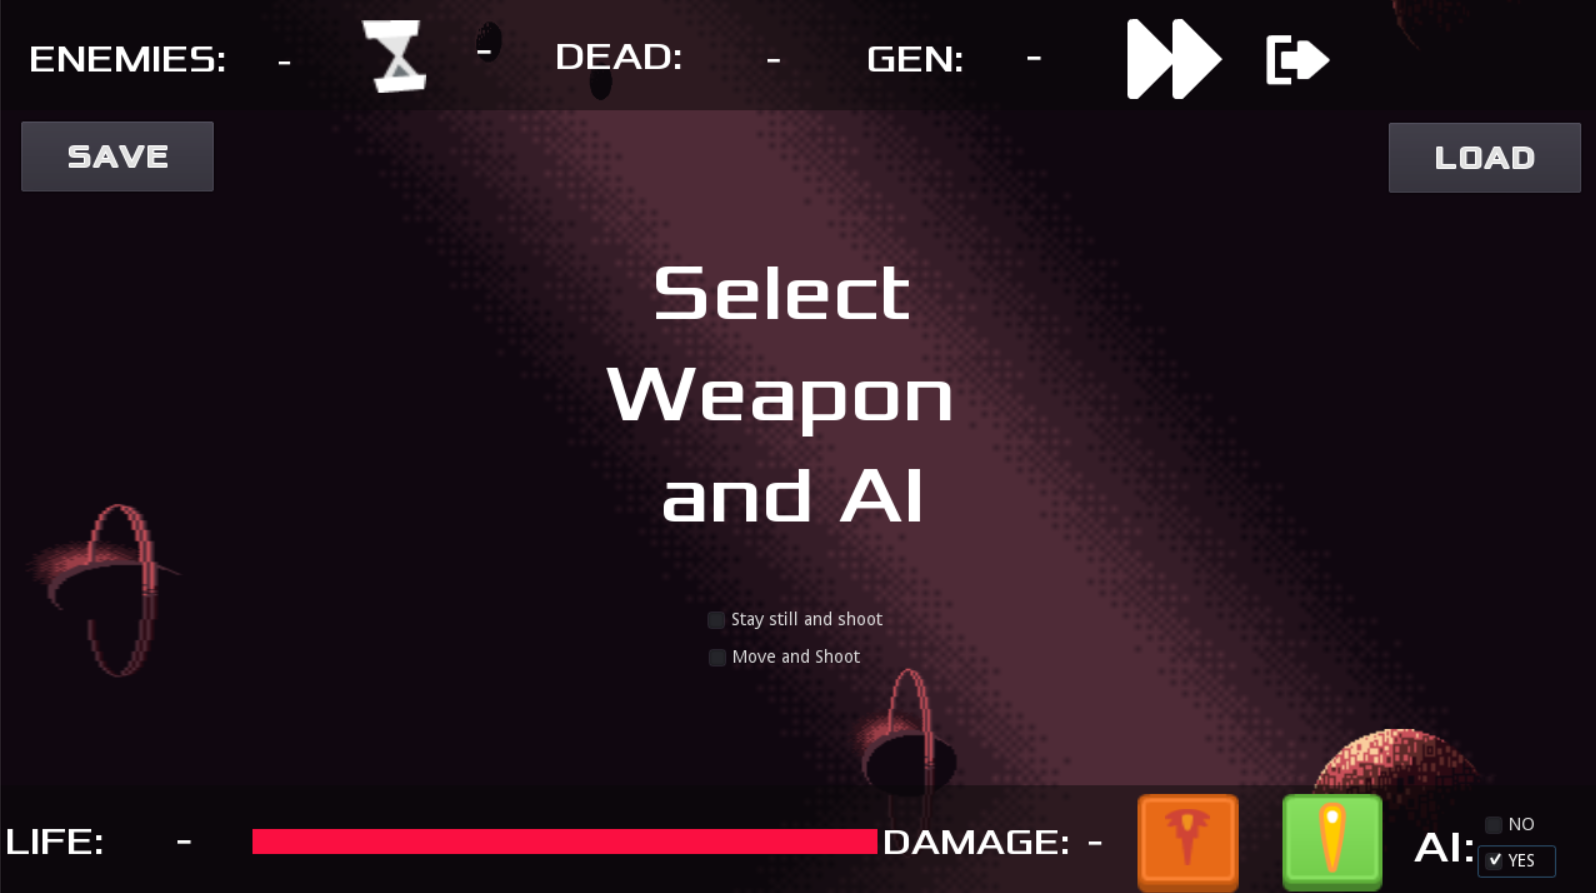
\includegraphics[width=\textwidth]{ss/Escolhendo player automatico.png}
  \caption{Opções de Player Automático. Imagem retirada do próprio jogo.\label{fig:ss-player-ai}}
\end{figure}


Existem 6 tipos de asteroides diferentes, presentes na Figura \ref{fig:ss-tipo-ast}. Cada tipo de asteroide possui 3 características, sendo elas velocidade, vida ou resistência e dano causado ao jogador, cujo os valores variam conforme o tipo, presentes na Tabela \ref{tab:ss-ast-dmg}. 

\begin{figure}
     \centering
     \begin{subfigure}[b]{0.15\textwidth}
         \centering
         
\includegraphics[width=\textwidth]{ss/inimigos.png}
         \caption{inimigos}
         \label{fig:ss-inimigos}
     \end{subfigure}
     \hfill
     \begin{subfigure}[b]{0.15\textwidth}
         \centering
         
\includegraphics[width=\textwidth]{ss/inimigo1.png}
         \caption{inimigo1}
         \label{fig:ss-inimigo1}
     \end{subfigure}
     \hfill
     \begin{subfigure}[b]{0.15\textwidth}
         \centering
         
\includegraphics[width=\textwidth]{ss/inimigo2.png}
         \caption{inimigo2}
         \label{fig:ss-inimigo2}
     \end{subfigure}

     \begin{subfigure}[b]{0.15\textwidth}
         \centering
         
\includegraphics[width=\textwidth]{ss/inimigo3.png}
         \caption{inimigo3}
         \label{fig:ss-inimigo3}
     \end{subfigure}
     \hfill
     \begin{subfigure}[b]{0.15\textwidth}
         \centering
         
\includegraphics[width=\textwidth]{ss/inimigo4.png}
         \caption{inimigo4}
         \label{fig:ss-inimigo4}
     \end{subfigure}
     \hfill
     \begin{subfigure}[b]{0.15\textwidth}
         \centering
         
\includegraphics[width=\textwidth]{ss/inimigo5.png}
         \caption{inimigo5}
         \label{fig:figure-inimigos}
     \end{subfigure}     
     \caption{Tipos de asteroides}
     \label{fig:ss-tipo-ast}
\end{figure}

\begin{table}[H]
\caption{Velocidade, dano e vida de cada asteroide no Space Shooter}
\begin{tabular}{c|ccc}
         & Velocidade & Dano & Vida   \\ \hline
inimigos & 500        & 20     &   50     \\
inimigo1 & 350        & 45     &   30     \\
inimigo2 & 470        & 50     &   40     \\
inimigo3 & 320        & 60     &   40     \\
inimigo4 & 550        & 20     &   60     \\
inimigo5 & 700        & 10     &   120      
\end{tabular}
\label{tab:ss-ast-dmg}
\end{table}

Após feitas as escolhas sobre o tipo de disparo que será utilizado e se o jogador vai mover a nave ou não, basta apertar o botão \textit{'Start'} para inicio do jogo. O jogador assim deve sobreviver às ondas de inimigos que aparecem de diferentes posições da tela. 

Caso seja atingido, a quantidade de dano que sofreu é exibida no campo \textit{'Damage'}. Por sua vez, quantidade de inimigos que apareceram enquanto o jogo ainda se desenrola é mostrada na barra superior na extrema esquerda, assim como outras informações como numero de asteroides que foram mortos e o números de gerações que foram enfrentadas. Há um botão para acelerar a velocidade do jogo, e outro que volta ao começo do jogo, caso o jogador não queria continuar ou tenha se arrependido das configurações iniciais que fez anteriormente, um exemplo de uma rodada do jogo encontra-se na Figura \ref{fig:ss-exemplo}.

\begin{figure}
  \centering
  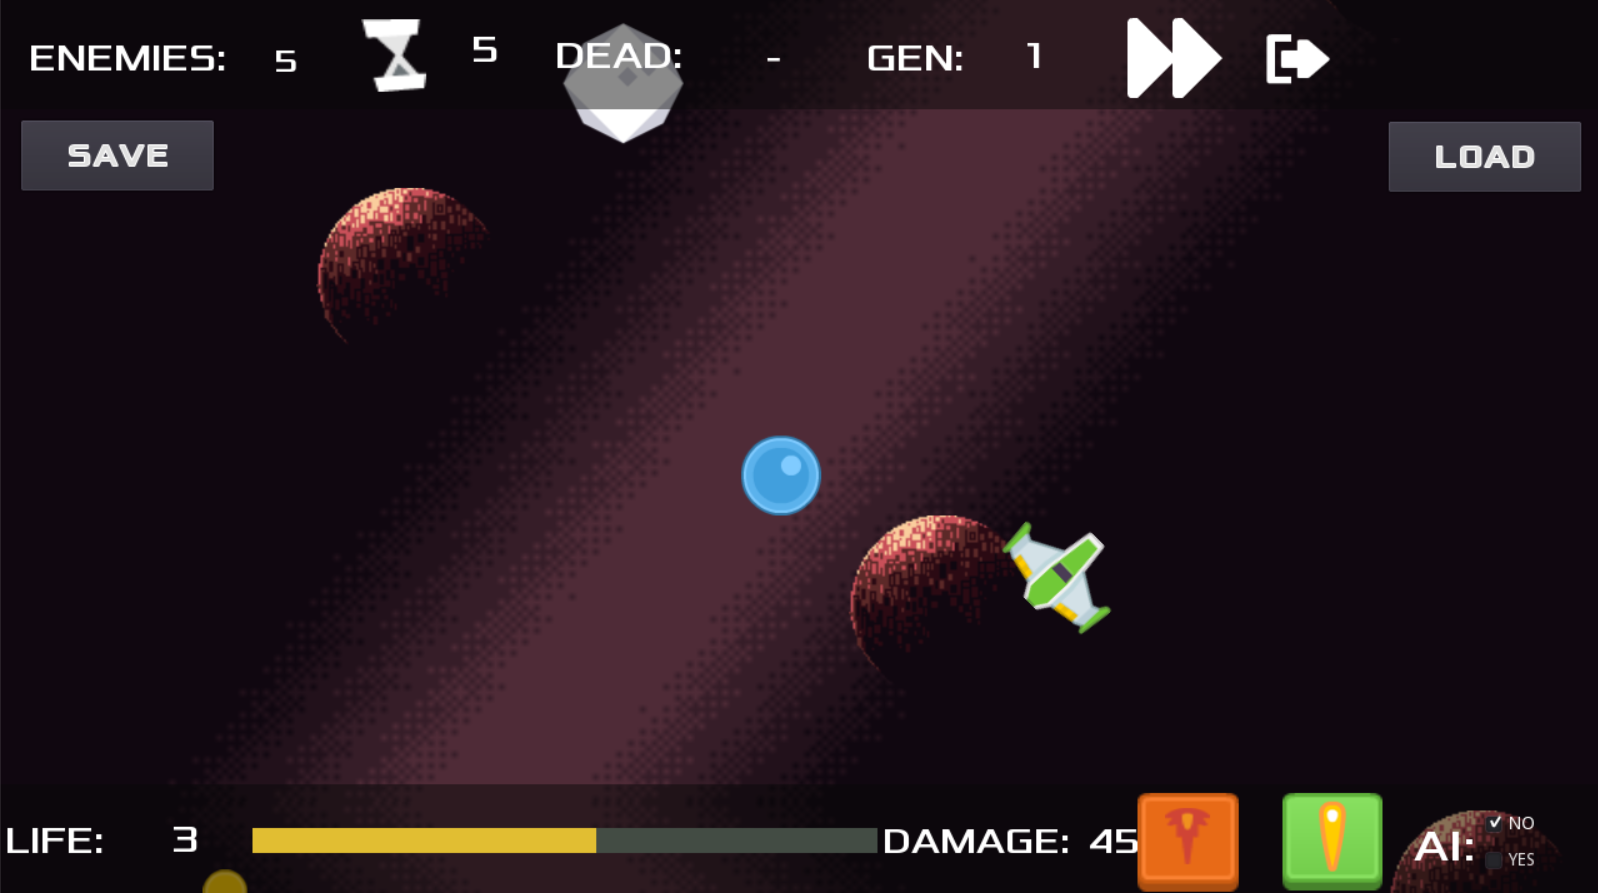
\includegraphics[width=\textwidth]{ss/Exemplo de jogo.png}
  \caption{Exemplo de uma rodada do jogo. Imagem retirada do próprio jogo.\label{fig:ss-exemplo}}
\end{figure}

O jogador começa com a sua barra de vida no valor total igual a 100. Caso chegue a zero 3 vezes o jogador morre e o jogo volta à tela inicial onde as configurações sobre a escolha de arma, por exemplo, devem ser feitas de novo. Ficam definidos os locais de \textit{spawn} de 1 até 6 na Figura \ref{fig:ss-positions}

\begin{figure}
  \centering
  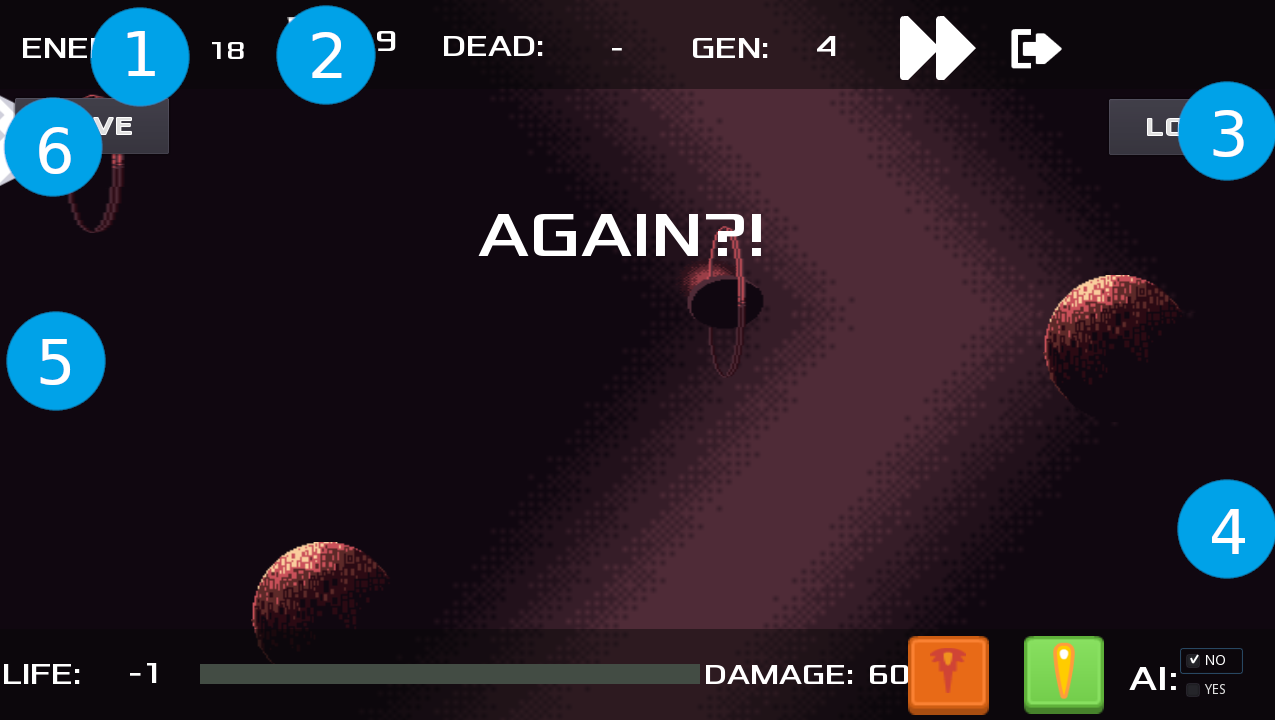
\includegraphics[width=\textwidth]{ss/ss_positions.png}
  \caption{Posições possíveis onde um asteroide pode surgir. Imagem retirada do jogo e editada.\label{fig:ss-positions}}
\end{figure}